% =====================================================================
% appA —— 附录 A Fredholm 算子的空间（原书 p.111–p.120）
%           ＋ 附录 A 章末评注
% =====================================================================
% [原文 p.111]
\chapter{Fredholm 算子的空间}

本附录用 Hilbert 空间来理解 $K(X)$\footnote{K. Jänich 独立得到这一结果（1964 年波恩大学学位论文）。译注：它以如下形式发表：K. Jänich, ‘Vektorraumbündel und der Raum der Fredholm-Operatoren’, \textit{Math. Ann.} \textbf{161} (1965) 129--142。}。这一点在与椭圆型算子的指标理论的联系中很有意义。

设 $H$ 是可分复 Hilbert 空间，$\cA(H)$ 是 $H$ 上所有有界算子组成的代数。给 $\cA$ 赋以范数拓扑。众所周知，$\cA$ 由此成为 Banach 环。特别地，$\cA$ 的单位群 $\cA^*$ 是开集。又由闭图像定理，若 $T\in\cA$ 是 $H$ 到 $H$ 的环同构，则它也是同胚。也就是说，$\cA$ 中存在 $T^{-1}$，因此 $T\in\cA^*$。

\begin{definition}{}
  称算子 $T\in\cA(H)$ 为 Fredholm 算子，若 $\Ker T$ 与 $\Coker T$ 都是有限维的。整数
  \[
    \dim\Ker T-\dim\Coker T
  \]
  称为 $T$ 的指标（index）。
\end{definition}

% [Tutor Note: 定义中两个维数都必须有限，指标才有意义；只要求其中一个有限并不够，因为 $\dim\Ker T$ 与 $\dim\Coker T$ 的差在扰动下才稳定。另注意此处的 index 是整数，与第 2 章中 $\operatorname{index}:[X,\cF]\to K(X)$ 的群值指标是同一概念的不同层级的推广。]

首先，注意 Fredholm 算子 $T$ 的像 $T(H)$ 是闭的。事实上，$T(H)$ 在 $H$ 中的余维数有限，所以可以找到有限维的代数补空间 $P$。于是，取 $j\colon P\to H$ 为包含映射，$T\oplus j\colon H\oplus P\to H$ 是满射，从而由闭图像定理，任意闭集的像都是闭的。特别地，$T(H)=(T\oplus j)(H\oplus0)$ 是闭的。

设 $\cF\subset\cA$ 为所有 Fredholm 算子组成的子空间。设 $T$, $S$ 为 Fredholm 算子，则
% [原文 p.112]
\[
  \dim\Ker(T\circ S)\le\dim\Ker T+\dim\Ker S,
\]
\[
  \dim\Coker(T\circ S)\le\dim\Coker T+\dim\Coker S
\]
成立。因此 $T\circ S$ 也是 Fredholm 算子。于是 $\cF$ 是具有结合乘法 $\cF\times\cF\to\cF$ 的拓扑空间。因此，对任意空间 $X$，从 $X$ 到 $\cF$ 的映射的同伦类集合 $[X,\cF]$ 是半群。本附录的主要目标是证明下述定理。

\begin{theorem*}{A.1}
  对任意紧空间 $X$，存在自然的同构映射
  \[
    \operatorname{index}\colon[X,\cF]\to K(X).
  \]
\end{theorem*}

% [Tutor Note: 这里是半群 $[X,\cF]$ 到群 $K(X)$ 的同构；$\cF$ 本身不连通，$[X,\cF]$ 只在同伦意义下成半群，故定理的“自然同构”中同构一词指半群同构。]

\para{备注} 当 $X$ 为一点时，这一定理意味着 $\cF$ 的连通分支由整数确定。这个整数正是前面定义的指标（index），定理 A.1 中的映射 index 是它的推广。

定理 A.1 断言 $\cF$ 是 K 理论对偶的分类空间，或者说是它的表示空间。与此密切相关的另一个分类空间如下得到。用 $\cK\subset\cA$ 表示所有紧算子。它是双侧闭理想，因此商 $\cB=\cA/\cK$ 也是 Banach 环。设 $\cB^*$ 为 $\cB$ 的单位群。它是拓扑群，因此对任意 $X$，$[X,\cB^*]$ 是群。于是第二个定理如下。

\begin{theorem*}{A.2}
  $\cB^*$ 是 K 理论的分类空间。也就是说，存在自然的群同构
  \[
    [X,\cB^*]\cong K(X).
  \]
\end{theorem*}

从下面的引理开始。它本质上是命题 1.3.2 的无穷维推广。
% [原文 p.113]
\begin{lemma*}{A.3}
  设 $T\in\cF$，$V$ 为 $H$ 的闭子空间，其余维数有限，且 $V\cap\Ker T=0$。此时存在 $T$ 在 $\cA$ 中的邻域 $U$，使对所有 $S\in U$ 满足下述条件：
  \begin{enumerate}[label=(\roman*),leftmargin=2.2em,itemsep=1pt,topsep=2pt]
    \item $V\cap\Ker S=0$；
    \item 给 $\bigcup_{S\in U}H/S(V)$ 赋以 $U\times H$ 的商空间拓扑后，它是 $U$ 上的平凡向量丛。
  \end{enumerate}
\end{lemma*}

\begin{proof}
  令 $W=T(V)^\perp$（$H$ 中 $T(V)$ 的正交补）。由于 $T\in\cF$ 且 $\dim H/V$ 有限，$\dim W$ 有限。这里对 $S\in\cA$ 定义
  \[
    \varphi_S\colon V\oplus W\to H
  \]
  为 $\varphi_S(V\oplus W)=S(V)+W$。于是 $S\mapsto\varphi_S$ 给出连续线性映射
  \[
    \varphi\colon\cA\to\mathcal L(V\oplus W,H),
  \]
  其中 $\mathcal L$ 表示赋以范数拓扑的所有连续线性映射的空间。现在 $\varphi_T$ 是同构映射。$\mathcal L$ 中全体同构映射，与 $\cA$ 中的 $\cA^*$ 一样，构成开集。因此存在 $T$ 在 $\cA$ 中的邻域 $U$，使所有 $S\in U$ 的 $\varphi_S$ 都是同构。由此显然得到条件 (i) 与 (ii)。
\end{proof}

\begin{corollary*}{A.4}
  $\cF$ 在 $\cA$ 中是开集。
\end{corollary*}

\begin{proof}
  在引理 A.3 中取 $V=(\Ker T)^\perp$ 即可。
\end{proof}

\begin{proposition*}{A.5}
  设 $X$ 紧，$T\colon X\to\cF$ 连续。此时存在闭且余维数有限的 $V\subset H$，使
  \begin{enumerate}[label=(\roman*),leftmargin=2.2em,itemsep=1pt,topsep=2pt]
    \item 对所有 $x\in X$，$V\cap\Ker T_x=0$
  \end{enumerate}
  成立。并且对这种 $V$
  \begin{enumerate}[label=(\roman*),leftmargin=2.2em,itemsep=1pt,topsep=2pt,start=2]
    \item 给 $\bigcup_{x\in X}H/T_x(V)$ 赋以 $X\times H$ 的商空间拓扑后，它是 $X$ 上的向量丛。
  \end{enumerate}
\end{proposition*}
% [原文 p.114]
\begin{proof}
  对每点 $x\in X$ 令 $V_x=(\Ker T_x)^\perp$，并令 $U_x$ 为引理 A.3 所给开集在 $T$ 下的原像。取 $K_i=U_{x_i}$ 为此开集族的有限覆盖。此时 $V=\bigcap_i V_{x_i}$ 满足条件 (i)。为证条件 (ii)，对每个 $T_x$ 应用引理 A.3，便知 $\bigcup_y H/T_y(V)$ 在 $x$ 附近局部平凡。因此 $\bigcup_{x\in X}H/T_x(V)$ 是向量丛。
\end{proof}

% [Tutor Note: (ii) 中的拓扑是 $X\times H$ 的商拓扑，并非各纤维上欧氏拓扑的简单并；这里“向量丛”的全部内容就是这一步局部平凡性，$\cA$ 上的范数拓扑恰好保证了 $\varphi_S$ 对 $S$ 连续。]

为简单起见，把命题 A.5 的向量丛 $\bigcup_{x\in X}H/T_x(V)$ 记作 $H/T(V)$。与有限维情形一样，映射 $p\colon X\times H\to H/T(V)$ 分裂。更确切地说，可以找到连续映射
\[
  \varphi\colon H/T(V)\to X\times H,
\]
它与到 $X$ 的投影可交换，且
\[
  p\circ\varphi=\text{恒等映射}
\]
成立。

构造 $\varphi$ 的一个办法，是用 $H$ 的度量把 $H/T(V)$ 映入 $T(V)$ 的正交补 $T(V)^\perp$。这在技术上不好用，因为必须验证 $T(V)^\perp$ 是向量丛。改用下述办法。依定义 $p$ 是局部地分裂的，所以取 $X$ 的有限开覆盖 $\{U_i\}$ 时，可以在 $U_i$ 上选到分裂 $\varphi_i$。此时 $\varphi_i-\varphi_j=\theta_{ij}$ 本质上是映射 $H/T(V)|_{U_i\cap U_j}\to(U_i\cap U_j)\times V$。取从属于此覆盖的单位分解 $\rho_i$，照例令
\[
  \theta_i=\sum\rho_j\theta_{ij},
\]
则 $\theta_i$ 在每个 $U_i$ 上都有定义。此时 $\varphi=\varphi_i-\theta_i$ 与 $i$ 无关，正是所求的分裂映射。

这样，对（$X$ 紧的）任意映射 $T\colon X\to\cF$ 都能定义 $\operatorname{index}T$。按命题 A.5 选取 $V$，令
% [原文 p.115]
\[
  \operatorname{index}T=[H/V]-[H/T(V)]\in K(X),
\]
其中 $H/V$ 表示平凡丛 $X\times H/V$。必须证明这一定义不依赖 $V$ 的选法。设 $W$ 是另一种选法，则 $V\cap W$ 也是这种选法，故不妨假定 $W\subset V$。但此时有向量丛的正合列
\[
  0\to V/W\to H/W\to H/V\to 0,
\]
\[
  0\to V/W\to H/T(W)\to H/T(V)\to 0.
\]
因此
\[
  [H/W]-[H/V]=[V/W]=[H/T(W)]-[H/T(V)]
\]
成立。

这个 $\operatorname{index}T$ 的定义显然是函子式的。也就是说，若 $f\colon Y\to X$ 连续，则
\[
  \operatorname{index}(T\circ f)=f^*\operatorname{index}T
\]
成立。这由“对 $T$ 选的部分空间 $V$ 同时也是对 $T\circ f$ 的部分空间”推出。

设 $T\colon X\times I\to\cF$ 是 $T_0$ 与 $T_1$ 之间的同伦，则 $\operatorname{index}T\in K(X\times I)$ 的限制是 $\operatorname{index}T_i\in K(X\times\{i\})$（$i=0,1$）。
\[
  K(X\times I)\to K(X\times\{i\})\cong K(X)
\]
是同构映射，这是已知的，因此
\[
  \operatorname{index}T_0=\operatorname{index}T_1
\]
成立。所以
\[
  \operatorname{index}\colon[X,\cF]\to K(X)
\]
是良定义的。

% [原文 p.116]
其次，必须证明“指标”是同态映射。设 $S\colon X\to\cF$ 与 $T\colon X\to\cF$ 连续。设 $W\subset H$ 是对 $T$ 选的部分空间。把 $S$ 换成同伦等价的映射 $\pi_W\circ S$（$\pi_W$ 表示到 $W$ 上的投影），便可假定 $S(H)\subset W$。这里对 $S$ 选取 $V\subset H$，它也是对 $T\circ S$ 的部分空间，于是得到 $X$ 上向量丛的正合列
\[
  0\to W/S(V)\xrightarrow{T}H/(T\circ S)(V)\to H/T(W)\to 0.
\]
因此
\begin{align*}
  \operatorname{index}(T\circ S)&=[H/V]-[H/(T\circ S)(V)]\\
  &=[H/V]-[W/S(V)]-[H/T(W)]\\
  &=[H/V]-[H/S(V)]+[H/W]-[H/T(W)]\\
  &=\operatorname{index}S+\operatorname{index}T
\end{align*}
成立。

这样便证明了 $\operatorname{index}\colon[X,\cF]\to K(X)$ 是同态映射，于是定理 A.1 的证明归结为下述命题。

\begin{proposition*}{A.6}
  半群的正合列
  \[
    [X,\cA^*]\to[X,\cF]\xrightarrow{\operatorname{index}}K(X)\to0
  \]
  成立。
\end{proposition*}

\begin{proof}
  先考虑指标为零的映射 $T\colon X\to\cF$。这意味着在 $K(X)$ 中
  \[
    [H/V]-[H/T(V)]=0
  \]
% [原文 p.117]
  成立。因此，两边加上平凡丛 $P$ 便得
  \[
    H/V\oplus P\cong H/T(V)\oplus P.
  \]
  同样地，若用满足 $\dim V/W=\dim P$ 的闭子空间 $W$ 替换 $V$，则
  \[
    H/W\cong H/T(W).
  \]
  这里，如前所述把 $X\times H\to H/T(W)$ 分裂，便得到
  \[
    \varphi\colon X\times H/W\to X\times H,
  \]
  它与到 $X$ 的投影可交换，并且在纤维上是线性的。设
  \[
    \Phi\colon X\to\mathcal L(H/W,H)
  \]
  为 $\varphi$ 附带的映射，则由 $\varphi$ 的构造，
  \[
    x\mapsto\Phi_x+T_x
  \]
  给出连续映射
  \[
    X\to\cA^*.
  \]
  而 $0\le t\le1$ 时，$T+t\Phi$ 给出连接 $T$ 与 $T+\Phi$ 的映射 $X\to\cF$ 的同伦。这样便证明了 $[X,\cF]$ 处的正合性。

  剩下只须证明 index 是满射。设 $E$ 是 $X$ 上的向量丛，$F$ 是使 $E\oplus F$ 同构于平凡丛 $X\times V$ 的补丛。用 $\pi_x\in\End(V)$ 表示到 $V$ 中对应于 $E_x$ 的子空间上的投影。选取正规正交基 $\{e_i\}$（$i=1,2,\dots$），便可定义指标为 $k$ 的标准算子 $T_k\in\cF$：
  \[
    T_k(e_i)=
    \begin{cases}
      e_{i-k} & (i-k\ge1\text{ 的情形}),\\
      0 & (\text{其余情形}).
    \end{cases}
  \]
  此时，映射
% [原文 p.118]
  \[
    S\colon X\to\cF(H\otimes V)\cong\cF(H)
  \]
  由 $S_x=T_{-1}\otimes\pi_x+T_0\otimes(1-\pi_x)$ 定义。对所有 $x$，$\Ker S_x=0$，且 $H\otimes V/S(H\otimes V)\cong E$ 成立。因此
  \[
    \operatorname{index}S=-[E].
  \]
  由 $T_k(x)=T_k$ 给出的常值映射 $T_k\colon X\to\cF$ 的指标是 $k$，从而
  \[
    \operatorname{index}(T_k\circ S)=k-[E].
  \]
  $K(X)$ 的所有元素都形如 $k-[E]$，所以此式说明指标是满射。命题证毕。
\end{proof}

这样，定理 A.1 由命题 A.6 与下述命题 A.7 推出。

\begin{proposition*}{A.7}
  $[X,\cA^*]=1$。
\end{proposition*}

这个命题属于 Kuiper，这里不重复其证明（细节见 Kuiper 的论文 \textit{Topology} \textbf{3} (1964) 19--30）。实际上，Kuiper 还证明了 $\cA^*$ 是可缩的。

% [Tutor Note: $\cA^*$ 可缩是无穷维 Hilbert 空间特有的现象，与有限维时酉群 $U(n)$ 的连通分支结构完全不同；正是这一可缩性使定理 A.1 的分类空间可以取 $\cF$ 而不必另作修正，Kuiper 定理是整篇附录的技术支柱。]

下面考虑定理 A.2 的证明。首先回想
\[
  1+\cK\subset\cF.
\]
这是紧算子理论中的标准结果，证明很简单。

\begin{proposition*}{A.8}
  设 $\pi\colon\cA\to\cB=\cA/\cK$ 为自然映射。此时
  \[
    \cF=\pi^{-1}(\cB^*)
  \]
  成立。
\end{proposition*}

\begin{proof}
  (a) 设 $T\in\cF$，用 $P$, $Q$ 分别表示到 $\Ker T$, $\Ker T^*$ 上的投影。此时 $T^*\circ T+P$ 与 $T\circ T^*+Q$ 都属于 $\cA^*$，
% [原文 p.119]
  从而它们在 $\pi$ 下的像属于 $\cB^*$。但 $P,Q\in\cK$，因此 $\pi(T^*)\pi(T)\in\cB^*$，$\pi(T)\pi(T^*)\in\cB^*$。这意味着 $\pi(T)\in\cB^*$。

  (b) 设 $T\in\pi^{-1}(\cB^*)$。也就是说，存在 $S\in\cA$，使 $S\circ T$ 与 $T\circ S$ 都是 $1+\cK\subset\cF$ 的元素。由于 $\dim\Ker T\le\dim\Ker(S\circ T)$ 以及
  \[
    \dim\Coker T\le\dim\Coker(T\circ S),
  \]
  故 $T\in\cF$。
\end{proof}

这样，定理 A.2 由定理 A.1 与下述一般引理推出（取 $L=\cA$、$M=\cB$、$U=\cB^*$ 应用）。

\begin{lemma*}{A.9}
  设 $\pi\colon L\to M$ 是 Banach 空间之间的连续线性映射，$\pi(L)$ 在 $M$ 中稠密，$U$ 是 $M$ 的开集。此时对任意紧空间 $X$，
  \[
    [X,\pi^{-1}(U)]\longrightarrow[X,U]
  \]
  是双射。
\end{lemma*}

\begin{proof}
  首先，若
  \[
    \pi\colon L\to M
  \]
  满足引理的条件，则对任意紧空间 $X$，诱导的映射
  \[
    \pi^X\colon L^X\to M^X
  \]
  也满足同样的条件。$L^X$、$M^X$ 是 Banach 空间，所以只须证明 $\pi^X(L^X)$ 在 $M^X$ 中稠密。设有 $f\colon X\to M$。必须构造 $g\colon X\to L$，使所有 $x\in X$ 满足 $\|\pi g(x)-f(x)\|<\varepsilon$。在 $f(X)$ 中选取 $a_1,\dots,a_n$，使它们的 $\frac{\varepsilon}{3}$ 邻域族 $\{U_i\}$ 覆盖 $f(X)$，并选取 $b_i$ 使 $\|\pi(b_i)-a_i\|<\frac{\varepsilon}{3}$，
% [原文 p.120]
  再令 $u_i(x)$ 为从属于覆盖 $\{f^{-1}U_i\}$ 的 $X$ 的单位分解，定义 $g\colon X\to L$ 为
  \[
    g(x)=\sum_i u_i(x)b_i.
  \]
  这就是所求的映射。

  于是，把 $\pi$ 换成 $\pi^X$，把 $U$ 换成（$M^X$ 中的开集）$U^X$，便知只须在 $X$ 是一点时证明引理。也就是说，只须证明
  \[
    \pi^{-1}(U)\to U
  \]
  诱导弧连通分支的双射。显然此映射是满射：即若 $P\in U$，则存在 $Q\in\pi(L)\cap U$，使线段 $PQ$ 完全含于 $U$ 中。下面证明此映射是单射。设 $P_0,P_1\in\pi^{-1}(U)$，$f\colon I\to U$ 是满足 $f(0)=\pi(P_0)$、$f(1)=\pi(P_1)$ 的道路。于是由前面证明的事实，存在 $g\colon I\to\pi^{-1}(U)$，使所有 $t\in I$ 满足
  \[
    \|\pi g(t)-f(t)\|<\varepsilon.
  \]
  若 $\varepsilon$ 足够小，则 $i=0,1$ 时连接 $\pi g(i)$ 与 $f(i)$ 的线段整体含于 $U$ 中。这意味着 $i=0,1$ 时连接 $g(i)$ 与 $P_i$ 的线段含于 $\pi^{-1}(U)$ 中。因此可以用 $\pi^{-1}(U)$ 中的道路连接 $P_0$ 与 $P_1$（参见下图）。证毕。
\end{proof}

\begin{figure}[htbp]
  \centering
  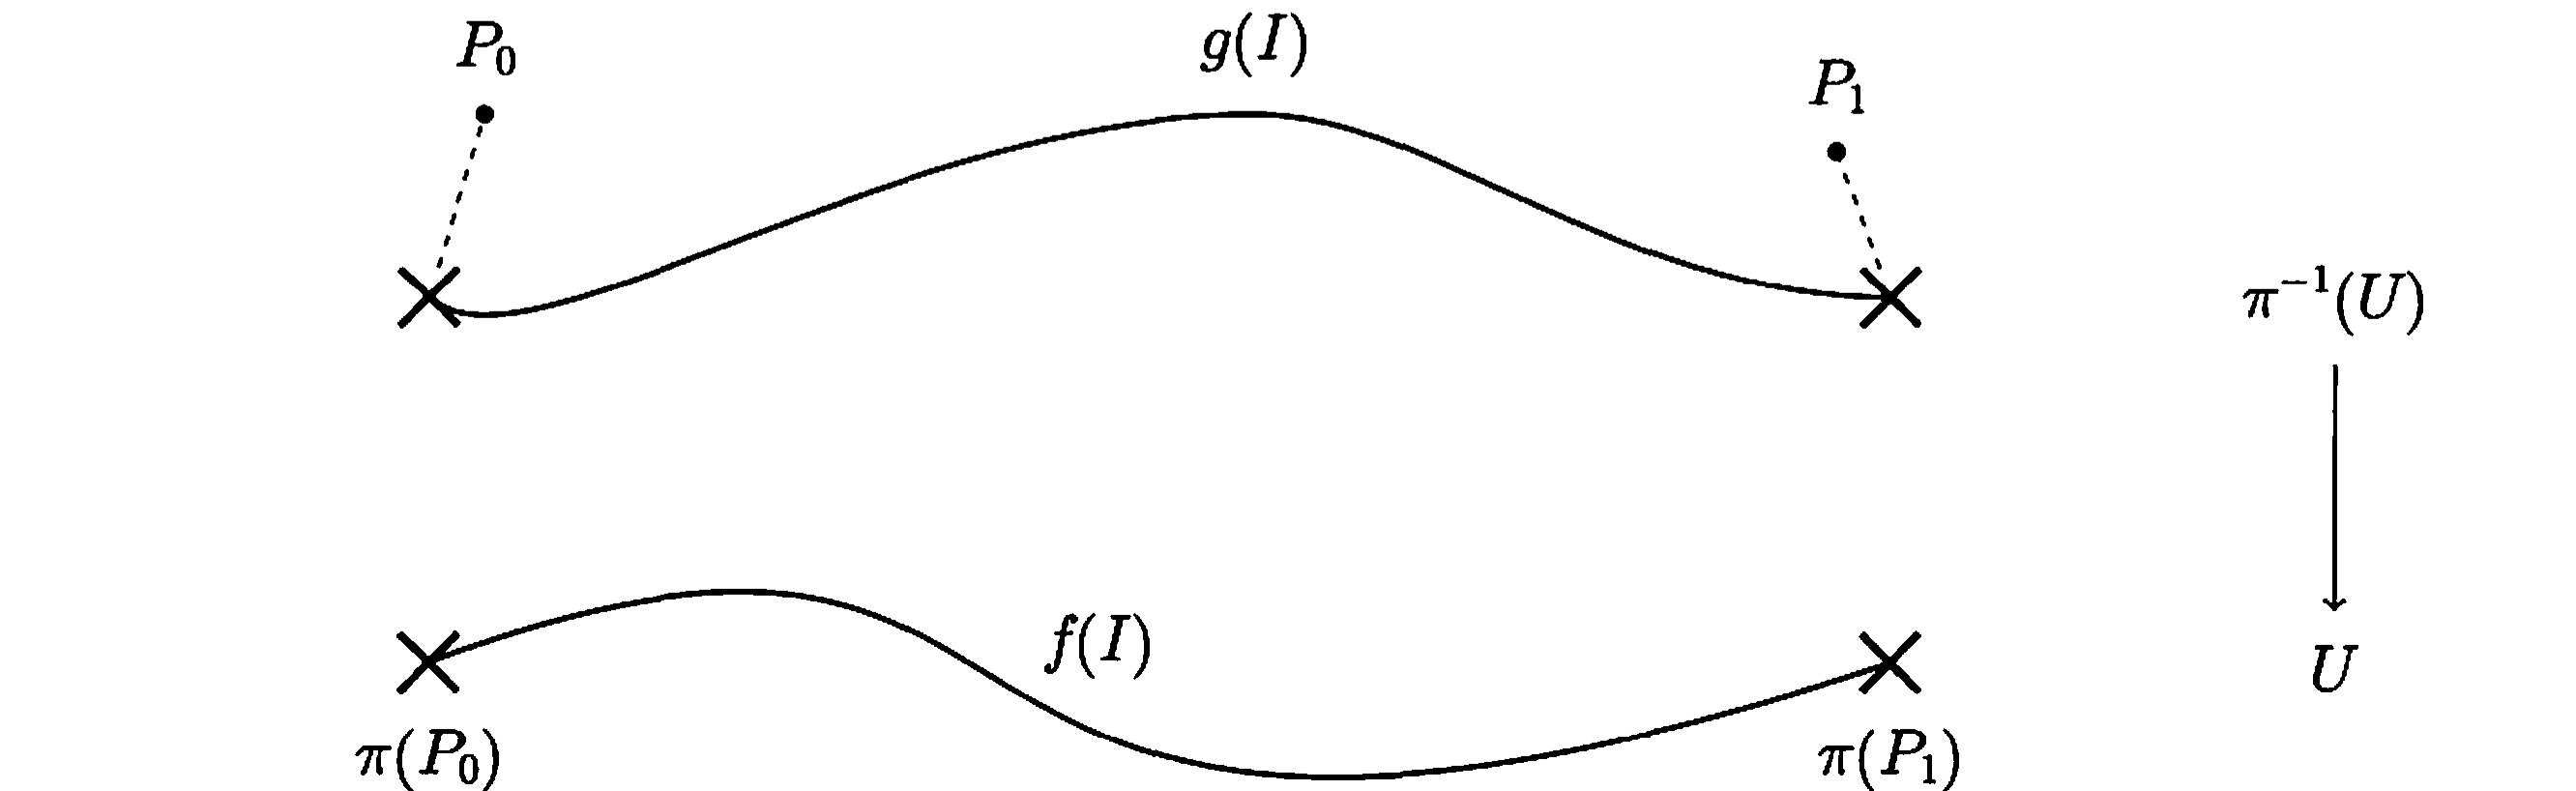
\includegraphics[width=0.92\textwidth]{figures/figA.1.png}
\end{figure}

\chapterreview{
本附录回答第 1、2 章遗留的一个自然问题：$K(X)$ 究竟可由什么样的空间分类？答案是 Fredholm 算子。这一结论把 K 理论从向量丛的组合构造中解放出来，使之与椭圆型算子的指标理论接轨；它也是全书唯一的“函数分析”章节，为后来 Atiyah–Singer 指标定理的叙述铺路。

脉络分两段。第一段（定理 A.1）取 $H$ 上全体有界算子代数 $\cA$ 中的 Fredholm 算子集 $\cF$：先证 $\cF$ 在 $\cA$ 中开，再证 $[X,\cF]$ 到 $K(X)$ 有自然的指标映射，且它是满同态（命题 A.6），核由 $\cA^*$ 的像填满（命题 A.7，即 Kuiper 定理）。第二段（定理 A.2）把 $\cF$ 换成商环 $\cB=\cA/\cK$ 的单位群 $\cB^*$，用一般引理 A.9 把“邻域上的同伦类”问题化归为单点的弧连通性，从而把定理 A.1 与命题 A.8 合成定理 A.2。

核心结论有两条：其一，$[X,\cF]\cong K(X)$，且同构由 $\operatorname{index}T=[H/V]-[H/T(V)]$ 给出，$V$ 的选取不影响结果；其二，$\cB^*$ 也是 K 理论的对偶分类空间，且 $\cF=\pi^{-1}(\cB^*)$。两条合起来说明：指标是 K 理论的普适不变量，而“无界方向”由紧算子商掉。

辨析上要注意三点。第一，$H/T(V)$ 的拓扑是 $X\times H$ 的商拓扑，不是纤维拓扑的并，命题 A.5 的全部内容是这一步的局部平凡性。第二，$\operatorname{index}T$ 的良定义依赖 $H/V\oplus P\cong H/T(V)\oplus P$ 的稳定化，这正是 $K$ 群而非向量丛半群的原因。第三，Kuiper 定理（$\cA^*$ 可缩）只对无穷维 $H$ 成立，不能与有限维酉群的结果类比。

评注：本附录把“分类空间”这一同伦论概念与“指标”这一分析概念并置，读者若只把它当作定理 A.1 的证明，会错过它的方法论意义——此后凡是要把 K 群实现为某个算子空间的同伦类，都沿用这一套路。附录 B 的幂算子是另一条推广路线，两者在指标定理处汇合。
}

% CHUNK appA DONE
